\chapter{Data and Methods}

This chapter will contain:

\begin{itemize}

    \item a short introduction of the scope of the project
    \item a short description of the dataset
    \item the statistical analysis of the data
    \item the description of the methods we will employ (stochastic logistic model, as in the article)
    
\end{itemize}


\section{Data}
We analize $10$ subjects (mother, father and their offspring of $8$ mice) during their whole lifespan. The length of the 
timeseries ranges from $524$ to $1044$ days. 


\begin{figure}
    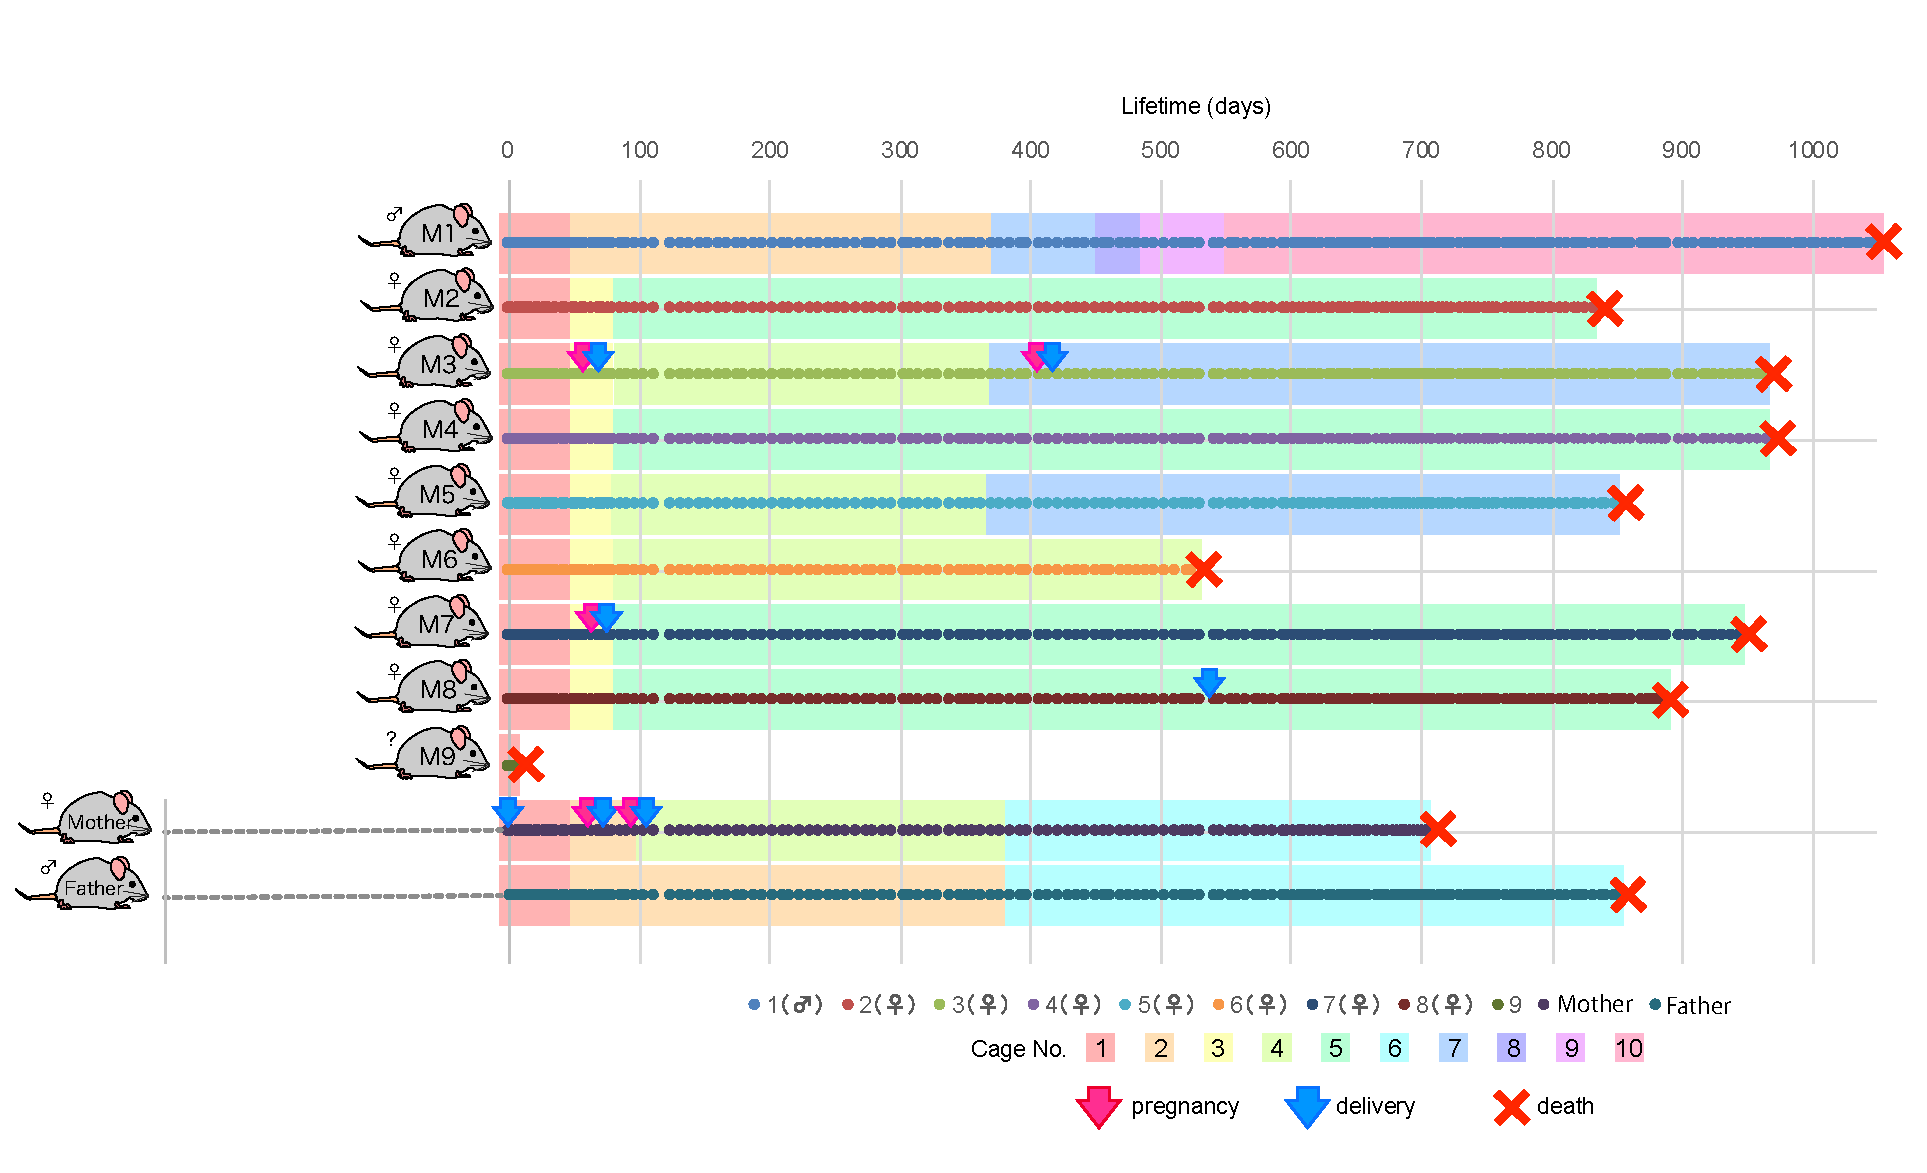
\includegraphics[width = 0.7\textwidth]{../../Figures/Chapter_1/fig_data.pdf}
    \caption{Schematics of data samples}
\end{figure}